\documentclass[10pt, a4paper]{scrartcl}
%\usepackage{a4wide}					%Platzintensiver
\usepackage[ngerman]{babel}	%Deutsche Silbentrennung
\usepackage[utf8]{inputenc}		%Damit kann man auch Umlaute direkt eintippen
\usepackage{textcomp}
\usepackage{amsmath}
\usepackage{amssymb}
\usepackage{color}
\usepackage{amsbsy}
\usepackage{mdwlist}
\usepackage{amsfonts}
\usepackage{amsthm}
\usepackage{graphicx}	%including images
\usepackage{fancyhdr}	%for editiable headers and footers
\usepackage{setspace} 	%for 1,5times row space
\usepackage[colorlinks,pdfpagelabels,pdfstartview = FitH,bookmarksopen = true,bookmarksnumbered = true,linkcolor = black,plainpages = false,hypertexnames = false,citecolor = black, linkcolor=black, menucolor=black, pagecolor=black, urlcolor=black] {hyperref}	
\usepackage{multirow}	%linebreak in Table
\usepackage{enumerate}
\usepackage{float}
\usepackage{colortbl}	%colorTables
\usepackage{framed}   %begin{framed}
\usepackage{longtable} %begin{longtable}
\usepackage{makeidx}
\usepackage[square]{natbib}
\usepackage{epigraph}
\usepackage{listings}
\lstset{
language=php,                		% choose the language of the code
basicstyle=\footnotesize,       % the size of the fonts that are used for the code
numbers=left,                   % where to put the line-numbers
numberstyle=\footnotesize,      % the size of the fonts that are used for the line-numbers
stepnumber=1,                   % the step between two line-numbers. If it's 1 each line will be numbered
numbersep=5pt,                  % how far the line-numbers are from the code
backgroundcolor=\color{white},
showspaces=false,
showstringspaces=false,
showtabs=false,
frame=single,
tabsize=4,
captionpos=t,
breaklines=true,
breakatwhitespace=false,
%escapeinside={\%*}{*\%}{//},  	% if you want to add a comment within your code
keywordstyle=\color{green}\bfseries,
commentstyle=\color{blue},
morecomment=[l]{//},
morecomment=[s]{/*}{*/},
morestring=[b]",
morestring=[d]’,
frame=tb
}
\lstset{index={}}

%	Eigenes PHP Syntax-HL
\usepackage{listings}
\usepackage{caption}
\usepackage{epigraph}
\usepackage[dvipsnames]{xcolor}
\lstset{%
basicstyle=\ttfamily\footnotesize\color{black},
commentstyle = \ttfamily\color{gray},
keywordstyle=\ttfamily\color{blue},
stringstyle=\color{red},
showspaces=false,               % show spaces adding particular underscores
showstringspaces=false, 
frame=single
}



\newcommand{\ownTitle}{Bachelorarbeit}
\newcommand{\ownTitleZ}{Leistungsuntersuchung von Webserveranwendungen und Optimierung auf Basis von Drupal 5 (am Beispiel von ITsax.de)}
\newcommand{\ownAutor}{Martin Schneider, HTW Dresden}



%%%%%%%%%%%%%%%%%%%%%%%%%%%%%%%%%%
%% HEAD AND FOOTLINES 
%%%%%%%%%%%%%%%%%%%%%%%%%%%%%%%%%%
\pagestyle{fancy}
\renewcommand{\sectionmark}[1]{\markboth{\thesection\ #1}{}}
\renewcommand{\subsectionmark}[1]{\markright{\thesubsection\ #1}}
\lhead[ \leftmark   ]{\textbf{\ownTitle}}
\rhead[\textbf{\ownTitleZ}]{\leftmark}
\lfoot[\thepage    ]{\scriptsize \textcopyright2011, \ownAutor}
\cfoot[]{}
\rfoot[\scriptsize \textcopyright2011, \ownAutor]{\thepage}

%%%%%%%%%%%%%%%%%%%%%%%%%%%%%%%%%%%%%%%
%  Macros
%%%%%%%%%%%%%%%%%%%%%%%%%%%%%%%%%%%%%%%%
\renewcommand{\footrulewidth}{0.5pt}
\newcommand{\cbox}{\includegraphics[width=0.2cm]{material/cbox.png} \ }
\definecolor{Gray}{rgb}{0.85,0.85,0.90}
% \setcounter{tocdepth}{2}	%kleineres TOC
\newcommand{\arr}{$ \Longrightarrow$}

\makeindex 	%start Aufzeichnun eines Stichwortverzeichnisses

%%%%%%%%%%%%%%%%%%%%%%%%%%%%%%%
%% Metainfos
%%%%%%%%%%%%%%%%%%%%%%%%%%%%%%%


\title{\ownTitle}
\author{\ownAutor}
\pdfinfo{
 /Title  (\ownTitle)
 /Author (\ownAutor)
 /Subject (\ownTitleZ)
 /Keywords()
}
\date{\today}
\onehalfspacing

\setlength{\epigraphwidth}{.8\textwidth}
%%%%%%%%%%%%%%%%%%%%%%%%%%%%%%%%%%%%%%%%%%
\begin{document}
 %\maketitle
 %\thispagestyle{empty}
\begin{center}
\begin{tabular}{lcr}
 \Large{HTW Dresden} & \verb|       |& \multirow{3}{*}{
\includegraphics[height=1.353cm]{material/htwlogo.jpg}} \\
 \Large{Fachbereich Informatik} &  & \\
%\ownTitleZ &  & \\
\end{tabular}\end{center}
\begin{center}


\end{center}
\begin{verbatim}


\end{verbatim}
\begin{center}
\textbf{\Huge{\ownTitle}}


\end{center}
\begin{verbatim}



\end{verbatim}
\begin{center}
\textbf{\LARGE{\ownTitleZ}}
\end{center}
\begin{verbatim}








\end{verbatim}
\begin{flushleft}
\begin{tabular}{lll}
\textbf{Autor:} & & Schneider, Martin\\
& & \\
\textbf{Seminargruppe} & & 08/041/02\\
& & \\
& & \\
\textbf{Betreuender Professor:} & & Prof. Vogt\\
& & \\
& & \\
\textbf{Datum:} & & \today\\

\end{tabular}

\end{flushleft}
 %\tableofcontents		%Inhaltsverzeichnis
 %\part{Einleitung}

\label{sec:intro}
\section{Motivation}

Der Autor dieser Arbeit absolvierte sein Pflichtpraktikum in der pludoni GmbH und war bis zum heutigen Tag als Werksstudent tätig.
\subsection{pludoni GmbH}
“pludoni kommt aus dem Esperanto und bedeutet weitergeben.” Das Unternehmen wurde 2008 von Dr. Jörg Klukas gegründet und hat als Ziel den regionalen Mittelstand bei der Kommunikation und Bewerbersuche durch Communities zu unterstützen. Die von pludoni gemanagten Communities heißen ITsax.de, ITmitte.de und MINTsax.de. Sie richten sich an Technologie-Firmen aus Sachsen beziehungsweise Mitteldeutschland und versuchen über zahlreiche Dienstleistungen einen Mehrwert für die beteiligten Unternehmen zu schaffen, im Allgemeinen gehören dazu:

\begin{itemize}
 \item Aggregation, Veröffentlichung und Weitergabe von Stellenanzeigen
 \item Organisation von regelmäßigen Community-Treffen zum Austausch der Unternehmen,
 \item Unterstützung und Beratung bei der Gestaltung Suchmaschinen-optimierter Inhalte und
 \item Infrastruktur zur gegenseitigen Empfehlung von Fachkräften und Lernenden.
\end{itemize}

\subsection{Ziel}
Alle Communities sind zum heutigen Zeitpunkt durch das Content Management System Drupal 5 realisiert. Drupal 5 ist mittlerweile schon vier Jahre alt und nicht mehr auf dem neuesten Stand was Web Performance betrifft. Es gibt Drupal mittlerweile schon in der Version 7.7 und es sind viele Verbesserungen in Sachen Geschwindigkeit eingeflossen. Leider ist es nicht trivial ein Upgrade durchzuführen, da viele Strukturen sich stark verändert haben. Aus diesem Grund wurde der Autor damit beauftragt die Möglichkeiten einer Drupal 5 Optimierung am Beispiel der ältesten Community ITsax.de zu ergründen und wenn vorhanden durchzuführen. Dabei soll ein Leitfaden entwickelt werden, anhand dessen Drupal 5 und allgemein Webseiten effizient optimiert werden können.

\section{Aufbau}
Die Arbeit ist in zwei Teile aufgeteilt. Der Theorieteil beschäftigt sich mit den Grundlagen der Web Performance beziehungsweise der Web Performance Optimierung. Im Praxisteil wird versucht die Webseite itsax.de auf Performancemängel zu untersuchen und sofern vorhanden sie zu beheben. 

 %\part{Theoretische Grundlagen}
\label{sec:theory}

\section{Web Performance}
\epigraph{``Human beings don’t like to wait. We don’t like waiting in line at a store, we don’t like waiting for our food at a restaurant, and we definitely don’t like waiting for Web pages to load.''}{Alberto Savoia}

Jeder Internetnutzer hat eine gewisse Toleranz gegenüber langsamen Webseiten. Wenn er auf einer Webseite zu lange warten muss, geht er zur Konkurrenz. Um dies zu verhindern ist Web Performance in der letzten Zeit ein immer wichtigeres Thema geworden. Aber was bedeutet Web Performance eigentlich? Zum einen gibt es die subjektive Performance, die ein Besucher beim Browsen einer Webseite empfindet. Gibt es für den Nutzer bemerkbare Wartezeiten oder reagiert die Webseite schneller als die Wahrnehmungsschwelle? Solche Kriterien sind sehr wichtig bei interaktiven Webseiten und haben auch zu dem Erfolg von Ajax beigetragen. Zum anderen kann man auch eine objektive Aussage über die Geschwindigkeit mit der eine Webseite generiert, ausgeliefert und beim Besucher im Browser angezeigt wird, treffen. 
\subsection{Usability}
Web Performance hat einen großen Einfluss auf die Bedienbarkeit von Webseiten. Ohne die starke Verbesserung ihrer Performance hätte Google mit GMail und ihren anderen Web Applikationen keinen Erfolg erzielen können. Nur wenn eine Anwendung auch in einer akzeptablen Geschwindigkeit auf Benutzerinteraktionen reagieren kann, hat sie eine Chance auf dem Markt zu bestehen. Es gibt einige Studien die sich mit Web Usability auseinandersetzen. Ergebnis waren unter anderem, dass langsamere Webseiten zu Vertrauensverlust, empfundenem Qualitätsverlust, niedrigeren Konversionsraten, höheren Bailoutraten und zu Nutzerfrustration führen.


%TODO quelle?
\subsection{Google Ranking}
Für (Internet-)Firmen ist es von immenser Bedeutung gefunden zu werden. Ein Großteil der Internetnutzer sucht Angebote über die Google-Suche. Google hat mit ihrer Initiative ``Let's make the web faster'' für viel Entwicklung und Aktivität im Bereich Web Performance gesorgt und arbeitet zielgerichtet weiter in diese Richtung. Dazu gehört seit  2008 Google AdWords und seit 2010 die Google Suche selbst. Dies stellt viele Unternehmen vor die Aufgabe, ihre Webseite zu optimieren und zu beschleunigen, um im Google Ranking konkurrenzfähig zu bleiben. Wie genau Google die Webseiten testet, ist nur zum Teil bekannt, da diese Informationen zu Googles Geschäftsgeheimnissen gehören. Es finden sich aber einige Fakten, die bei der Optimierung für die Google Suche, im Bereich Web Performance, helfen können.
Bekannt ist dass der Google Suchmaschinen Bot nichts mit der Geschwindigkeitsmessung zu tun hat und Google nur Daten von echten Nutzern, die die Google Toolbar in ihrem Browser installiert haben, nutzt. Leider sind Daten nur für Internet Explorer ab Version 6 und Firefox ab Version 2 verfügbar. Als Kriterium für die Bewertung wird die Onload Zeit gemessen. Das bedeutet, dass das verzögerte Nachladen von Inhalten zu einem besseren Ergebnis führt, da dadurch die Onload Zeit verbessert wird. Wenn eine Webseite für Google Optimiert werden soll, muss also auch die Performance mit berücksichtigt werden. Performance ist aber nur ein Teil der Google Bewertung, es sollten also aktuelle und gut strukturierte Inhalte nicht hinter die Performance gestellt werden.

%TODO bild?
%%http://www.webperformancetoday.com/2011/08/05/faqs-google-seo-search-ranking-website-speed/

\subsection{Serverlast}
Eine umfassende Verbesserung der Auslieferungszeiten von Webseiten hat direkten Einfluss auf die Serverperformance. Dies ist leicht in einem Experiment feststellbar, wie folgende Überlegung zeigt: Wenn eine Webseite nur noch die Hälfte der Zeit benötigt, um ausgeliefert zu werden, hat man doppelt soviel Auslieferungskapazität zur Verfügung. Das spart Kosten für Server und Traffic. Außerdem ermöglichen Caching und Optimierungen einen Großteil an Prozessorlast einzusparen, der dann für andere Aufgaben zur Verfügung steht. Besonders wichtig ist die Performance in Momenten besonders hoher Zugriffszahlen, zum Beispiel wenn eine Webseite in einem prominenten Newsportal erwähnt wird. Oftmals bricht dann die Webseite zusammen, weil die Administratoren nicht mir solch einem Ansturm gerechnet haben. Erwähnenswert ist das Newsportal www.heise.de auf dem regelmäßig davon gesprochen wird, es wurde eine Webseite ``geheist''. Noch problematischer wird es wenn ein Unternehmen Ziel krimineller Aktivitäten wird. Aktuelle zu beobachten ist das bei den Angriffen des Miner-Botnetzes auf mehrere deutsche Webseiten. Um sich vor solchen Distributed Denial of Service angriffen schützen zu können, ist eine Performante Webseite sehr wichtig um genug Ressourcen für Firewalls und andere Gegenmaßnahmen zur Verfügung zu haben.

\section{Performance Bottlenecks}
Performance Bottlenecks oder auch Performance Flaschenhälse genannt, beschreiben Schwachpunkte in einem Datenverarbeitungssystem. Auf Web Performance angewendet, kann man das in clientseitige Probleme und serverseitige Probleme unterteilen.
\subsection{Clientseitige Bottlenecks}
\subsubsection{Netzwerkverbindung}Die Netzwerkverbindung kann auf zwei Ebenen für Probleme sorgen. Zum einen kann eine hohe Latenz für langsame auch auf Serverseite auftreten, aber da kann mit mehr Servern und besseren Anbindungen Abhilfe geschafft werden. Viel problematischer wird das auf der Clientseite da selten bekannt ist mit welcher Anbindung Nutzer eine Webseite besuchen werden.%TODO bild netzwerk
Da in Deutschland der Breitbandausbau noch lange kein Stadium erreicht hat, der es Webseitenbetreibern erlauben würde auf die Größe der Webseite die sie an ihre Betrachter ausliefern keinen Wert zu legen. Der Breitbandausbau peilt für 2011 eine 100 prozentige Versorgung mit 1 Mbit/s an und so sind noch viele Nutzer sind mit langsamen Internetzugängen im Internet unterwegs. 

\subsubsection{Browser}
Als Schnittstelle zwischen Mensch und Webseite ist der Browser ein besonders kritischer Punkt und muss bei Web Performanceanalysen besonders beachtet werden. Zum einen müssen die verschiedenen Browserfamilien, mit ihren Eigenheiten und Problemen und zum anderen die Tatsache das ein Browser nur so schnell arbeiten kann, wie der Computer auf dem er ausgeführt wird zulässt, beachtet werden. Problemzonen sind:
\begin{itemize}
  \item Anzahl von zu berechnenden DOM-Elementen
  \item Javascript Ausführungszeiten
  \item Anzahl benötigter HTTP Zugriffe
  \item 

\end{itemize}

\subsubsection{DOM Elemente}
\subsection{Serverseitig}
So gut wie jede Website nutzt mittlerweile eine Datenbank, diese können verschiedenster Natur sein zum Beispiel:
\begin{itemize}
\item SQLite
\item MySQL
\item MSSQL
\item PostGreSQL
\item 
\end{itemize}
Oft sind diese Datenbanken ein Schwachpunkt für die Web-Performance, da meistens Daten von der Festplatte gelesen werden müssen und komplexe Abfragen viel Zeit in Anspruch nehmen können.
\subsubsection{Datenbankabfragen}

\subsubsection{Skriptausführung}
\subsubsection{Skriptkompilierung}

\section{Technologiestack und Optimierungsmöglichkeiten}
Im Rahmen dieser Bachelorarbeit werden verschiedenste Technologien verwendet und auf ihnen aufbauende Werkzeuge zu Hilfe genommen. Um zu verstehen wo Probleme lokalisiert sind und wie solche Schwachstellen zu finden sind muss man sich mit dem vorhandenem Technologiestack auseinandersetzen und ihn analysieren.
\begin{description}
  \item[Server] Ein Server ist ein Computer, der Informationen und Dienste für andere Computer zur Verfügung stellt
  \item[Betriebssystem] Die Software die auf dem Server läuft. In der pludoni GmbH wird das Linuxderivat Debian eingesetzt.
  \item[Datenbank] Als Datenbank wird eine strukturierte Sammlung von Daten bezeichnet. MySQL ist hier die erste Wahl.
  \item[Web Server] Der Web Server ist für die zuverlässige Auslieferung von Webseiten zuständig. Er beantwortet die Anfragen die die Nutzer mit dem Browser stellen. Apache2 wird dafür in der pludoni GmbH eingesetzt.
  \item[PHP] PHP ist eine Programmiersprache, die es Web Entwicklern ermöglicht dynamische Webseiten zu programmieren.
  \item[Drupal] Drupal ist ein Framework, welches in PHP geschrieben ist und viele direkt nutzbare Funktionen mitbringt. Dazu gehören unter anderem Administrationsoberflächen, Newsaggregatoren, Veröffentlichungsabläufe für Artikel und Blogbeiträge sowie Suchmaschinenoptimierungen. Außerdem ermöglicht Drupal die Installation weiterer, durch Nutzer entwickelte, Module. Dadurch wird eine fast unbegrenzte Funktionsvielfalt ermöglicht. Im vorliegenden Fall wird Drupal in der Version 5 eingesetzt.
  \item[Client] Im Browser der Nutzer kommt am Ende HTML an, dies wird durch Drupal generiert und vom Webserver ausgeliefert. Dabei werden Bilder verarbeitet Javascript Programme ausgeführt und andere Elemente wie Flashapplikationen und Videos berechnet. 
\end{description}

\subsection{Server}
\subsection{PHP}
\subsection{Drupal (5)}
Drupal ist ein Content-Management-System, dass heißt es ermöglicht dem Nutzer eine dynamische Webseite zu erstellen ohne spezielle Programmierkenntnisse zu besitzen. 
\subsection{Benchmark - Werkzeuge}
\subsection{Debugger / Profiler}
\section{Methoden der Web-Performance Optimierung}
Die Methoden zur Leistungssteigerung können wie im Technologiestack untergliedert werden und jedes Element muss für sich betrachtet werden.

\begin{description}
  \item[Server] Der einzige Parameter der am Server verbessert werden kann ist seine Leistung, dass heißt Datendurchsatz und Rechengeschwindigkeit. Dies geschieht durch CPU Upgrades oder Arbeitsspeichererweiterung. Weitergehend kann man die Festplattenzugriffsgeschwindigkeiten durch RAID Verbünde und neue Technologien wie SSD Speicher verbessern. 
  \item[Betriebssystem] Ansatzpunkte für Verbesserungen auf Betriebssystemebene sind Memory-Mapping, dass heißt Speicherbereiche die normalerweise auf der Festplatte liegen werden in den Arbeitsspeicher umgelagert um die Latenzen zu verringern. Dies wird genutzt um Caches zu beschleunigen, die normalerweise von der Festplatte lesen.
  \item[Datenbank] Auf Datenbankebene kann im Fall von MySQL nur beschränkt optimiert werden. Zum einen sind Indizes anzulegen bei häufig genutzten Tabellen und zum anderen kann man MyISAM statt InnoDB nutzen um Performanter zu sein.
  \item[Web Server] Optimierungen am Webserver sind sehr schwierig da die Webserver Performance hauptsächlich von der Serverleistung abhängt. Die Anzahl der gleichzeitigen Zugriffe wird maßgeblich durch den verfügbaren Arbeitsspeicher und die verfügbare Bandbreite eingeschränkt.
  \item[PHP] 
  \item[Drupal] 
  \item[HTML] 
\end{description}


%
\part{Praxisteil}

Versuchsaufbau:

Testplattform: pludoni Server eq4
Prozessor: Intel® Core™ i7-920
Arbeitsspeicher: 8 GB DDR3 RAM
Festplatten: 2 x 750 GB SATA-II HDD (Software-RAID 1)
Netzwerkverbindung: 100Mbit

Livesystem: pludoni Server 
Prozessor: Intel® Core™2 Quad CPU Q6600 @ 2.4 Ghz
Arbeitsspeicher: 4 GB DDR3 RAM
Festplatten: 2 x 750 GB SATA-II HDD (Software-RAID 1) %TODO aktualisieren
Netzwerkverbindung: 100Mbit

Testclient: Virtualbox
Firefox 5

Testobjekt:
Itsax Startseite


Ausgangszustand:
Sreeram Ramachandran ein Software Engineer bei der Firma Google hat eine Analyse über 4.2 Milliarden Seiten veröffentlicht. Diese ist im Rahmen der Initiative ``Let's make the web faster'' entstanden und zeigt häufige Fehlerquellen und ungenutztes Potential auf. Die durchschnittliche Webseite hat laut Ramachandran 320 KB Größe, 44 verschiedene Ressourcen und es werden nur 66\% der komprimierbaren Inhalte tatsächlich komprimiert.
Itsax.de hat 106 Ressourcen und 444 KB an Daten. Schon anhand dieser zwei Zahlen lässt sich eine vergleichsweise schwache Leistung vorhersehen. Besonders die Anzahl an verschiedenen Ressourcen deutet auf Missstände hin, da Parallelisierung von Zugriffen nur bis zu einem bestimmten Grad möglich ist. Die Time to First Byte(TtFB) von 674ms bezeichnet die Zeit die vergeht bis der Webbrowser die ersten Daten empfängt, dass bedeutet aber noch nicht das der Nutzer schon Inhalte präsentiert bekommt. Die Inhalte werden erst angezeigt nachdem die Time to Start Render(TtSR) vergangen ist, der Nutzer muss demnach ungefähr zwei Sekunden warten bis die Webseite im Browser anfängt sich aufzubauen. Die Load Time(LT) bezeichnet dann die Zeit die vergeht bis die Seite komplett dargestellt wird und der Benutzer sie ohne Einschränkungen bedienen kann. Es können  aber auch nach der LT noch Inhalte nachgeladen werden, wie zum Beispiel gestreamte Videos oder andere asynchrone Inhalte. Diese nachgeladenen Inhalte wirken sich aber nicht mehr Negativ auf die User Experience aus, solange sie im Rahmen bleiben und nicht wichtige Teile der Webseite wie zum Beispiel das Hauptmenü noch per Flash geladen werden müssen. Die Anzahl der DOM Elemente bezeichnet alle vom Browser zu verarbeitenden Objekte und ist ein Indikator für die Komplexität der Webseite, je mehr Elemente also vorhanden sind desto länger muss der Browser die Positionierung und Darstellung berechnen. Die Inhalte auf der Seite Itsax.de sind in Abbildung ? dargestellt, einmal im Bezug auf Größe und einmal aufgeschlüsselt nach der Anzahl der benötigten Requests um die Inhalte vom Server anzufordern. 

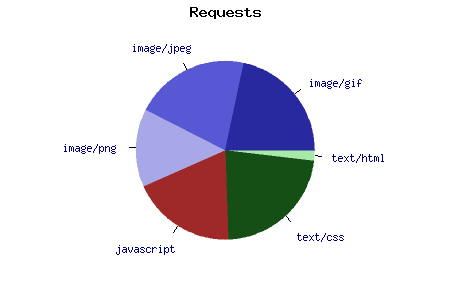
\includegraphics[scale=0.5]{material/start_request_pie.png}
\begin{tabbing}
Request \quad\= blablabla \quad\= \kill
\textbf{Typ} 	 \> \textbf{Anzahl} \\
text/css	 \>	24 	\\
image/gif	 \>	23 	\\
image/jpeg	 \>	22 	\\
javascript	 \>	20 	\\ 
image/png	 \>	15 	\\
text/html	 \>	2 	\\

\end{tabbing}

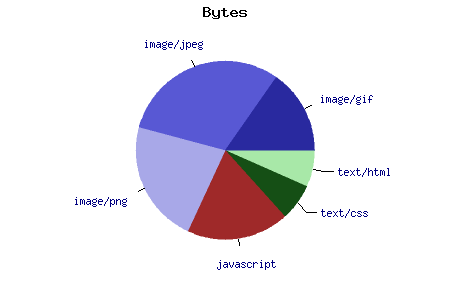
\includegraphics[scale=0.5]{material/start_byte_pie.png}

%http://code.google.com/intl/de/speed/articles/web-metrics.html

%TODO Bilder einfügen aus materials

text/css24
image/gif	22
image/jpeg	22
javascript	20
image/png	15
text/html	3

image/jpeg	142251
image/png	101428
javascript	84758
image/gif	73378
text/css	30222
text/html	29917
Ausgangssituation:
Server Software:        Apache/2.2.16
Server Hostname:        itsax.it-jobs-und-stellen.de
Server Port:            80

Document Path:          /
Document Length:        65218 bytes

Concurrency Level:      1
Time taken for tests:   18.182 seconds
Complete requests:      50

Write errors:           0
Total transferred:      3266726 bytes
HTML transferred:       3239226 bytes
Requests per second:    2.75 [\#/sec] (mean)
Time per request:       363.640 [ms] (mean)
Time per request:       363.640 [ms] (mean, across all concurrent requests)
Transfer rate:          175.46 [Kbytes/sec] received




Mit APC aktiviert:
Server Software:        Apache/2.2.16
Server Hostname:        itsax.it-jobs-und-stellen.de
Server Port:            80

Document Path:          /
Document Length:        64842 bytes

Concurrency Level:      1
Time taken for tests:   11.681 seconds
Complete requests:      50

Write errors:           0
Total transferred:      3261730 bytes
HTML transferred:       3234230 bytes
Requests per second:    4.28 [\#/sec] (mean)
Time per request:       233.620 [ms] (mean)
Time per request:       233.620 [ms] (mean, across all concurrent requests)
Transfer rate:          272.69 [Kbytes/sec] received

Mit Drupal Cache in normal Einstellung:
Server Software:        Apache/2.2.16
Server Hostname:        itsax.it-jobs-und-stellen.de
Server Port:            80

Document Path:          /
Document Length:        65005 bytes

Concurrency Level:      1
Time taken for tests:   2.082 seconds
Complete requests:      50
Failed requests:        0
Write errors:           0
Total transferred:      3276900 bytes
HTML transferred:       3250250 bytes
Requests per second:    24.02 [\#/sec] (mean)
Time per request:       41.638 [ms] (mean)
Time per request:       41.638 [ms] (mean, across all concurrent requests)
Transfer rate:          1537.09 [Kbytes/sec] received

Mit Drupal Cache in aggressiv Einstellung:



Test von Serverunabhängigen verbesserungen:
über das Analysetool von webpagetest.org
Testverfahren: 10 konsekutive Tests (maximum) der Durschnittlichste Testlauf wird betrachtet
Teststandort Frankfurt a. M.
Browser: IE9
Connection: DSL 1,5 Mbps / 50ms RTT
Only First View




Load Time: 3.728
Time to First Byte: 0.674s 	
Time to Start Render: 2.002s
\#DOM Elements: 855 	
\#Requests: 106
Bytes In: 444 KB
%http://www.webpagetest.org/result/110809_BH_198S4/


Im folgenden Abschnitt werden die eingesetzten Methoden dargestellt und ihre Auswirkungen auf die Webperformance der Seite ITsax.de dargestellt. 
JS Aggregation und Minifizierung mit dem Javascript Aggregation Modul:
Aggregation und Minifizierung sind Verfahren, die in der Webperformance Optimierung häufig eingesetzt werden. Für das Drupal 5 System gibt es fertige Module die diese Aufgabe übernehmen. Das Modul interveniert innerhalb des Drupal Kerns und ersetzt die Javascripts, die vorher direkt so ausgegeben wurden wie sie die Module lieferten, durch eine einzelne, das heisst aggregierte Version, die optional minifiziert werden kann. Diese Minifizierung wird natürlich genutzt und spart einige KB. Minifizierung wird ermöglicht durch die Nutzung von JSmin https://github.com/rgrove/jsmin-php/. JSmin ist ein Filter der unter anderem Kommentare entfernt und mehrere Leerzeichen zu einem zusammenfasst. Durch die Nutzung dieser Methode konnten 11 HTTP Abfragen und 11 KB an Datenvolumen eingespart werden.
Load Time: 3.658s
Time to First Byte: 0.595s
Time to Start Render: 1.915s
\#DOM Elements: 844 	
\#Requests: 95 %!
Bytes In: 432 KB
%http://www.webpagetest.org/result/110809_Z1_198TK/

CSS Aggregation und Komprimierung:
Analog zur Javascript Optimierung kann man auch die CSS Aggregation betrachten. Es werden durch Zusammenfassung der einzelnen CSS Dateien HTTP Abfragen eingespart. Wie man an der gesunkenen Anzahl der Requests sehen kann, wurden 21 Abfragen nur durch Zusammenfügen der einzelnen CSS Dateien zu einer einzigen eingespart. Durch die Bereinigung beziehungsweise Komprimierung werden dabei außerdem 17 Kb an überflüssigen Zeichen entfernt. 
Load Time: 3.577s
Time to First Byte: 0.649s
Time to Start Render: 1.577s
\#DOM Elements: 834 	
\#Requests: 85 %!
Bytes In: 427 KB
%http://www.webpagetest.org/result/110809_XB_198VE/

Drupal Boost Module:
Load Time: 3.233s
Time to First Byte: 0.172s %!
Time to Start Render: 1.473s
\#DOM Elements: 856 	
\#Requests: 106 %!
Bytes In: 444 KB
%http://www.webpagetest.org/result/110809_AP_198XJ/

Bildoptimierungen mit jpegoptim und OptiPNG verlustfrei!: 
Bilder und Grafiken bieten oft großen Optimierungsspielraum, zum einen durch die richtige Auswahl der Dateiformate und zum anderen durch Komprimierung der Bilder. Da es auf www.ITsax.de nicht nur statische Inhalte gibt, sondern auch durch Communitymitglieder und Communitymanager eingestellte Inhalte verwaltet werden müssen, sollte eine nachträgliche Qualitätsoptimierung der hochgeladenen Bilder durchgeführt werden. Um dies umzusetzen sind die Programme OptiPNG und jpegOptim zu empfehlen. Auf jeden Fall sollte eine verlustfreie Komprimierung durchgeführt werden, da die Bilder in diesem Fall nur an Dateigröße verlieren und die Bildqualität unberührt bleibt. Da es sich bei beiden Programmen um Kommandozeilenprogramme handelt kann man ihre Anwendung leicht automatisieren. Mit dem Linuxbefehl find, der praktischerweise eine Möglichkeit Befehle auszuführen besitzt, kann man direkt die entsprechenden Dateien an die Optimierer übergeben. Diese Aktionen können dann über einen Cronjob periodisch jede Nacht ausgeführt werden. Die Befehle sehen dann wie folgt aus: 
find . -name "*.png" -exec optipng -o7 {} \;
find . -name "*.jpg" -exec jpegoptim {} \;

%%http://optipng.sourceforge.net/
%%http://www.kokkonen.net/tjko/projects.html

Load Time: 3.640
Time to First Byte: 0.636s %!
Time to Start Render: 1.894s
\#DOM Elements: 855 	
\#Requests: 106 %!
Bytes In: 429 KB % 15kb gespart
%http://www.webpagetest.org/result/110809_C4_1999C/

Bildoptimierungen mit OptiPNG verlustfrei und mit jpegoptim verlustbehaftet! 50\% kompression:
find . -name "*.png" -exec optipng -o7 {} \;
find . -name "*.jpg" -exec jpegoptim {} \;

Load Time: 3.255s
Time to First Byte: 0.669s %!
Time to Start Render: 1.908s
\#DOM Elements: 855 	
\#Requests: 106 %!
Bytes In: 371 KB % 73kb gespart
%http://www.webpagetest.org/result/110809_15_199GY/

Drupal 5 Fehler bei umgefärbten Themes:
Das Framework Drupal 5 benutzt Themes zu Gestaltung der Oberfläche, um diese farblich anpassen zu können wurde das Color Modul installiert, welches Themeveränderungen ermöglicht. Dadurch das das Theme nur kopiert und die Farben geändert werden entstehen bei diesem Vorgang unnötige Duplikate die beim Laden der Seite mitgeschleppt werden. Um diese zu Entfernen wird einfach das Standardtheme durch das Modifizierte ersetzt. Dafür müssen  nur noch einige Pfade in der style.css angepasst werden und man spart in dem fall von ITsax.de 4 kb, was immerhin ca 1\% der übertragenen Datenmenge ausmacht.
händisch gemergte styles
style auf standard setzen
vorher die images und das geänderte stylesheet kopieren
Load Time: 3.626s
Time to First Byte: 0.629s %!
Time to Start Render: 1.890s
\#DOM Elements: 854 	
\#Requests: 104 %!
Bytes In: 440 KB % 4kb gespart
%http://www.webpagetest.org/result/110809_SZ_19APH/

Theme Bilder Spriten:
Spriting wurde ursprünglich in der Videospielentwicklung verwendet um Bilder in der Grafikspeicher zu laden. In der Webentwicklung ist es eine effektive Technik um Bilder ohne mehrfachen Overhead zu laden. Beim Spriting wird aus vielen einzelnen Bildern ein einziges Bild erstellt, dass anstelle der vielen Bilder geladen wird. Um die Bilder dann noch einzeln Anzeigen zu können werden CSS Befehle genutzt, die es ermöglichen die Größe und die Position eines Bildausschnittes anzuzeigen. 
Load Time: 3.707
Time to First Byte: 0.669s %!
Time to Start Render: 1.968s
\#DOM Elements: 855 	
\#Requests: 103 
Bytes In: 443 KB 
%http://www.webpagetest.org/result/110810_FZ_19GBA/

Verschiedene Module von Startseite entfernen:
Um zu überprüfen welchen Einfluss verschiedene, im Netzwerkgraphen auffällige Module auf die Gesamtperformance haben werden sie Testweise komplett deaktiviert. So kann man entscheiden bei welchen Module zusätzlicher Programmieraufwand lohnenswert ist.
Partnerslideshow:
Load Time: 2.695s
Time to First Byte: 0.636s %!
Time to Start Render: 1.838s
\#DOM Elements: 790 	
\#Requests: 80 
Bytes In: 276 KB
%http://www.webpagetest.org/result/110810_JT_19HS5/

facebook fenster:
Load Time: 3.478s
Time to First Byte: 0.668s %!
Time to Start Render: 1.966s
\#DOM Elements: 779 	
\#Requests: 95 
Bytes In: 406 KB 
%http://www.webpagetest.org/result/110810_63_19HZT/

Jobleiste deaktiviert:
Load Time: 3.367s
Time to First Byte: 0.617s %!
Time to Start Render: 1.709s
\#DOM Elements: 822 	
\#Requests: 94 
Bytes In: 411 KB
%http://www.webpagetest.org/result/110810_4F_19J8H/

Umprogrammierung verschiedener Module: Um die langsamen Module weiterhin nutzen zu können muss eine Lösung gefunden werden, die es ermöglicht Inhalte nachzuladen nachdem die Seite komplett geladen wurde. Um das zu erreichen kann man mit der Hilfe von Javascript bestimmte DOM Elemente über einen Timeoutbefehl erst nachdem der Browser gemeldet hat er hat die Seite fertig geladen, die Inhalte nachladen.
Partnerslideshow:
Load Time: 2.749s (3.794)
Time to First Byte: 0.626s %!
Time to Start Render: 1.842s
\#DOM Elements: 855 	
\#Requests: 82 (107)
Bytes In: 284 KB (395)
%http://www.webpagetest.org/result/110810_3Z_19MRE/

facebook fenster:
Load Time: 3.411s (4.258)
Time to First Byte: 0.576s %!
Time to Start Render: 1.848s
\#DOM Elements: 857
\#Requests: 95 (106)
Bytes In: 406 KB (444)
%http://www.webpagetest.org/result/110810_AJ_19N72/

Partneranzeigen:
Load Time: 3.871s (5.759s)
Time to First Byte: 0.669s %!
Time to Start Render: 2.255s
\#DOM Elements: 857 	
\#Requests: 105 (108)
Bytes In: 417 KB (448)
%http://www.webpagetest.org/result/110815_N6_1AWKT/1/details/


Komplett alle Maßnahmen:

%\section{Code-Metriken}
        \subsection{Notwendigkeit von Code Metriken}
        \subsection{Überblick über Code-Metriken und Skalen}
        \subsection{Testabdeckung}

 \part{Praxisteil}

\section{Versuchsaufbau}
Der Optimierungsversuch kann leider nicht auf dem Livesystem durchgeführt werden, da dass die Stabilität beeinträchtigen würde. Deswegen wurde ein Entwicklungssystem genutzt, um die verschiedenen Methoden zu analysieren. Dass Entwicklungssystem ist eine neuere Anschaffung der pludoni GmbH und dadurch im Vergleich zum Livesystem leistungsfähiger. Dadurch wird sich das Endergebnis, wenn es nach dem Abschluss der Arbeit auf das Livesystem übertragen wurde in seinen Kenndaten unterscheiden. Trotz alledem werden die Verbesserungen relativ zum Testsystem proportional ausfallen. 

\begin{itemize}
 \item Testplattform: pludoni Server eq4
  \item Prozessor: Intel® Core™ i7-920
  \item Arbeitsspeicher: 8 GB DDR3 RAM
  \item Festplatten: 2 x 750 GB SATA-II HDD (Software-RAID 1)
  \item Netzwerkverbindung: 100Mbit
  \item Server Software: Apache/2.2.16
  \item Server Hostname: itsax.it-jobs-und-stellen.de
  \item Server Port: 80
\end{itemize}

\section{Testverfahren}
Das Testen von Web-Performance hat sich in den letzten Jahren stetig weiterentwickelt. Eine Zeit lang galten sogenannte Backbonetests als das Non-Plus-Ultra. Nach dem aber immer deutlicher wurde, dass die tatsächlichen Ergebnisse sich stark von den Erwartungen unterschieden suchte man nach Alternativen. Der verlässlichste Test ist natürlich direkt beim Kunden beziehungsweise der Zielgruppe. Da es oft schwierig ist diese Tests durchzuführen, sollte zumindest mit ähnlichen Vorraussetzungen getestet werden.
\subsection{Servertest}
Die rein serverseitigen Optimierungen wurden mit ab getestet. ab, das für apache bench steht, wurde entwickelt um Apache Server zu testen. Es analysiert wie lange ein Server braucht um Webseiten auszuliefern und wieviele Anfragen er pro Sekunde befriedigen kann, ohne das es zu Ausfällen kommt. ab führt 50 Anfragen hintereinander auf die Ressource aus, und berechnet dann anhand der Ergebnisse die durchschnittliche Antwortzeit. Der Kommandozeilenbefehl der zum Testen genutzt wurde war denkbar einfach:
\begin{lstlisting}[language=bash,label=ab mit Paramtern,caption=ab mit Parametern]
ab -n 50 -c 1 http://itsax.it-jobs-und-stellen.de/
\end{lstlisting}

\subsection{Browsertest}
Browsertests sind eine sehr komplizierte Angelegenheit, da es zum einen sehr viele Verschiedene Browser gibt und zum Anderen diese Browser in den verschiedensten Umgebungen ausgeführt werden. Ein Netbook zum Beispiel wird eine Webseite immer langsamer Darstellen, als ein Desktop-PC der neuesten Generation. Man kann natürlich am eigenen Computer Test durchführen, dafür gibt es auch Programme wie Firebug und YSlow die auch Verbesserungsvorschläge liefern können. Da aber möglichst Objektiv getestet werden soll ist es von Vorteil eine standardisierte und automatisierte Umgebung zu nutzen. Für diesen Zweck bietet sich WebPagetest an. Es wurde ursprünglich für den internen Gebrauch bei AOL entwickelt, steht aber seit 2008 unter der BSD Lizenz und kann somit frei genutzt werden. Es ist eine umfassende Testsuite für Webseiten. Besonders die verschiedenen Analysen die automatisch durchgeführt werden sind positiv hervorzuheben. Es kann die Webseite nach den Google Page Speed Kriterien Bewerten und ausführliche Inhaltsanalysen, aufgeschlüsselt nach MIME Typen, liefern. Zusätzlich wird ein sehr hilfreiches Wasserfalldiagramm erzeugt und für jedes Element der Webseite ein Performance Review erstellt. Darin werden unter anderem Kriterien wie Kompression und Caching betrachtet. Als besonderes Feature gibt es noch einen Videovergleich, in dem man Webseiten gegeneinander antreten lassen kann. Man kann WebpageTest sowohl selbst installieren als auch externe Anbieter nutzen. In diesem Fall wird www.webpagetest.org mit folgenden Paramtern genutzt:
\begin{itemize}
  \item 10 konsekutive Tests (maximum) 
  \item Standort des Clients: Frankfurt a. M.
  \item Browser: IE9
  \item Connection: DSL 1,5 Mbps / 50ms RTT
  \item Only First View
\end{itemize}
\subsection{Andere Analyse Verfahren}
Profiling und Debugging auf Codeebene wurden nur sporadisch eingesetzt, da sie den Anwendungsfall Webseite nur eingeschränkt betreffen. Durch Caching kann der Server zum großen Teil vollständig entlastet werden und die Codeausführungszeit kann eliminiert werden. Bei Anwendungsfällen die kein Caching erlauben, wie zum Beispiel eine Suche oder eine Applikation, ist es sehr hilfreich diese Tools zu verwenden. Sie ersparen viel Arbeit, da die Problemstellen schnell ausgemacht werden können. Von Hand diese Arbeiten durchzuführen ist in kleinen Projekten sehr mühsam und in großen Projekten fast unmöglich. Jeder Entwickler sollte solche Programme in seinem Repertoire haben.

\section{Ausgangszustand}
Sreeram Ramachandran ein Software Ingenieur der Firma Google hat eine Analyse über 4.2 Milliarden Seiten veröffentlicht. Diese ist im Rahmen der Initiative ``Let's make the web faster'' entstanden und zeigt häufige Fehlerquellen und ungenutztes Potential auf. Die durchschnittliche Webseite hat laut Ramachandran 320 kB Größe, 44 verschiedene Ressourcen und es werden nur 66\% der komprimierbaren Inhalte tatsächlich komprimiert. 
Itsax.de hat 106 Ressourcen und 444 kB an Daten. Schon anhand dieser zwei Zahlen lässt sich eine vergleichsweise schwache Leistung vorhersehen. Besonders die Anzahl an verschiedenen Ressourcen deutet auf Missstände hin, da Parallelisierung von Zugriffen nur bis zu einem bestimmten Grad möglich ist. Die Time to First Byte(TtFB) von 674ms bezeichnet die Zeit die vergeht bis der Webbrowser die ersten Daten empfängt, dass bedeutet aber noch nicht das der Nutzer schon Inhalte präsentiert bekommt. Die Inhalte werden erst angezeigt nachdem die Time to Start Render(TtSR) vergangen ist, der Nutzer muss demnach ungefähr zwei Sekunden warten bis die Webseite im Browser anfängt sich aufzubauen. Die Load Time(LT) bezeichnet dann die Zeit die vergeht bis die Seite komplett dargestellt wird und der Benutzer sie ohne Einschränkungen bedienen kann. Es können  aber auch nach der LT noch Inhalte nachgeladen werden, wie zum Beispiel gestreamte Videos oder andere asynchrone Inhalte. Diese nachgeladenen Inhalte wirken sich aber nicht mehr Negativ auf die User Experience aus, solange sie im Rahmen bleiben und nicht wichtige Teile der Webseite wie zum Beispiel das Hauptmenü noch per Flash geladen werden müssen. Die Anzahl der DOM Elemente bezeichnet alle vom Browser zu verarbeitenden Objekte und ist ein Indikator für die Komplexität der Webseite, je mehr Elemente also vorhanden sind desto länger muss der Browser die Positionierung und Darstellung berechnen. Mit 855 DOM Elementen ist ITsax.de da schon auf der komplexeren Seite, was zu einem Großteil Drupal anzurechnen ist, welches durch seine gute Konfigurierbarkeit Einbußen in    Die Inhalte auf der Seite Itsax.de sind in Abbildung ? dargestellt, einmal im Bezug auf Größe und einmal aufgeschlüsselt nach der Anzahl der benötigten Requests um die Inhalte vom Server anzufordern. Die folgenden Ergebnisse wurde mit dem Analysetool webpagetest.org ermittelt. Leicht zu erkennen ist, dass der HTML Anteil sowohl bei der Größe als auch bei Anzahl der HTTP Anfragen eine Untergeordnete Rolle spielt. Nicht vergessen werden darf aber die Zeit die der Server benötigt um den HTTP Code zu generieren. Dies kann man sehr gut in einem Wasserfalldiagramm erkennen, in dem der Start des Ladevorgangs hervorgehoben wurde. Bevor der Initiale GET Request abgeschlossen ist, weiss der Browser noch nicht welche Ressourcen er laden muss und es können noch keine anderen Aktionen ausgeführt werden.
\begin{figure}[htbp]
  \centering
  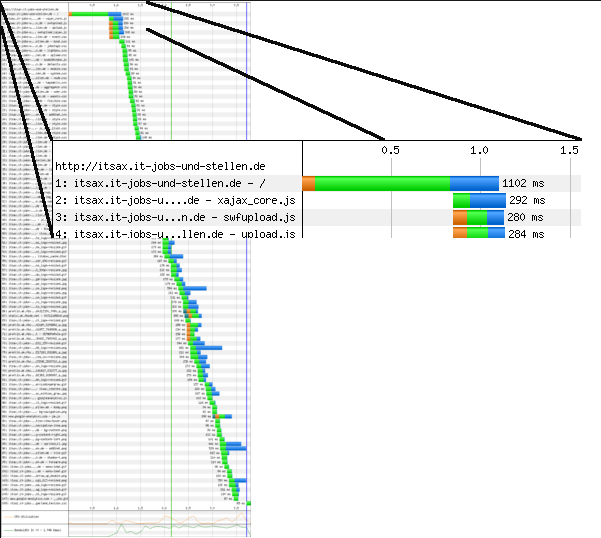
\includegraphics[scale=0.5]{material/start_waterfall_edited.png}
  \caption{Wasserfalldiagramm: Ausgangszustand}
  \label{fig:startwaterfall}
\end{figure}
\begin{figure}[htbp]
  \centering
  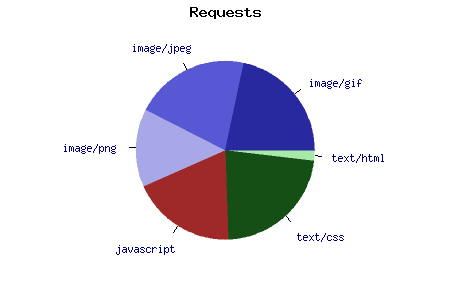
\includegraphics[scale=0.5]{material/start_request_pie.png}
  \caption{HTTP Anfragen}
  \label{fig:startrequest}
\end{figure}

\begin{figure}[htbp]
  \centering
  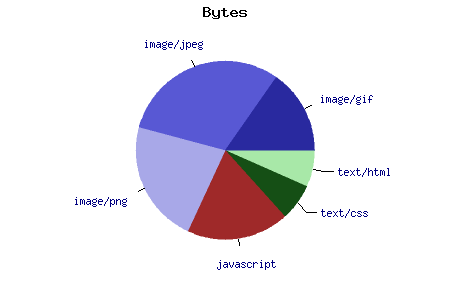
\includegraphics[scale=0.5]{material/start_byte_pie.png}
  \caption{Größe der Inhalte}
  \label{fig:startbyte}
\end{figure}

Load Time: 3.728
Time to First Byte: 0.674s 	
Time to Start Render: 2.002s
\#DOM Elements: 855 	

\begin{tabbing}
Request \quad\= blablabla \quad\= \kill
\textbf{Typ} 	 \> \textbf{Anzahl} \\
text/css	 \>	24 	\\
image/gif	 \>	23 	\\
image/jpeg	 \>	22 	\\
javascript	 \>	20 	\\ 
image/png	 \>	15 	\\
text/html	 \>	2 	\\
\end{tabbing}

\begin{tabbing}
Request \quad\= blablabla \quad\= \kill
\textbf{Typ} 	 \> \textbf{Byte} \\
image/jpeg	\>142251\\
image/png	\>101428\\
javascript	\>84758\\
image/gif	\>73378\\
text/css	\>30222\\
text/html	\>29917\\

\end{tabbing}
%http://code.google.com/intl/de/speed/articles/web-metrics.html
\begin{lstlisting}[language=bash,label=Ausgabe von ab,caption=Ausgabe von ab]
Server Software:        Apache/2.2.16
Server Hostname:        itsax.it-jobs-und-stellen.deDocument Path:          /
Document Length:        65218 bytes

Concurrency Level:      1
Time taken for tests:   18.182 seconds
Complete requests:      50

Write errors:           0
Total transferred:      3266726 bytes
HTML transferred:       3239226 bytes
Requests per second:    2.75 [#/sec] (mean)
Time per request:       363.640 [ms] (mean)
Time per request:       363.640 [ms] (mean, across all concurrent requests)
Transfer rate:          175.46 [kBytes/sec] received
\end{lstlisting}




\section{Implementierung und Test der einzelnen Methoden}
Im folgenden Abschnitt werden die eingesetzten Methoden dargestellt und ihre Auswirkungen auf die Webperformance der Seite itsax.de dargestellt. 
In diesem Abschnitt werden alle Methoden die vom Autor, nach der Analyse des Ausgangszustands, für möglicherweise sinnvoll befunden wurden getestet. Die Methode wird jeweils mit dem Startwert verglichen und der Aufwand wird eingeschätzt.
\subsection{APC} Als allererste Maßnahme wurde ein PHP Opcode Cache ausprobiert. Opcode Caches speichern die Ergebnisse vorangegangener Operationen und kann so beim nächsten Aufruf direkt die Ergebnisse ausliefern, wenn Anfrage gleichgeblieben ist. Solche Systeme sind immer zu empfehlen, da sie normalerweise keinerlei Probleme bereiten und alle PHP Anfragen beschleunigen.Aktuell gibt es mehrere verschiedene sogenannte PHP Beschleuniger unter ihnen nimmt aber APC eine führende Position ein. Hauptsächlich weil es der zuverlässigste unter den nicht-kommerziellen Caches ist.Ab PHP Version 5.4 wird er in PHP schon enthalten sein. Die Installation von APC ist auf einigermaßen aktuellen Linux Servern auch denkbar einfach. Das PHP Pear Framework, was oft schon installiert ist, erlaubt es mit einigen wenigen Befehlen einen funktionierenden Opcode Cache zu installieren. 
\begin{lstlisting}[language=bash,label=Installation von APC,caption=Installation von APC]
apt-get install php-pear
pecl install apc
\end{lstlisting}
Nach der Installation wurde die Antwortzeit des Apacheservers gemessen und es kam zu folgendem Ergebnis. Statt 363 ms wurden nur noch 233 ms benötigt, eine Verbesserung um 36\% und es können 4,28 Anfragen je Sekunde bearbeitet werden gegenüber vorher nur 2,75. Alles unter der Prämisse das es keine multiplen Anfragen gibt. 
\begin{lstlisting}[language=bash,label=Ausgabe von ab,caption=Ausgabe von ab]
Server Software:        Apache/2.2.16
Server Hostname:        itsax.it-jobs-und-stellen.de
Server Port:            80

Document Path:          /
Document Length:        64842 bytes

Concurrency Level:      1
Time taken for tests:   11.681 seconds
Complete requests:      50

Write errors:           0
Total transferred:      3261730 bytes
HTML transferred:       3234230 bytes
Requests per second:    4.28 [\#/sec] (mean)
Time per request:       233.620 [ms] (mean)
Time per request:       233.620 [ms] (mean, across all concurrent requests)
Transfer rate:          272.69 [kBytes/sec] received
\end{lstlisting}
\subsection{Drupal Cache}
\begin{lstlisting}[language=bash,label=Ausgabe von ab,caption=Ausgabe von ab]
Server Software:        Apache/2.2.16
Server Hostname:        itsax.it-jobs-und-stellen.de
Server Port:            80

Document Path:          /
Document Length:        65005 bytes

Concurrency Level:      1
Time taken for tests:   2.082 seconds
Complete requests:      50
Failed requests:        0
Write errors:           0
Total transferred:      3276900 bytes
HTML transferred:       3250250 bytes
Requests per second:    24.02 [\#/sec] (mean)
Time per request:       41.638 [ms] (mean)
Time per request:       41.638 [ms] (mean, across all concurrent requests)
Transfer rate:          1537.09 [kBytes/sec] received
\end{lstlisting}

%http://www.webpagetest.org/result/110809_BH_198S4/


\subsection{JS Aggregation und Minifizierung mit dem Javascript Aggregation Modul}
Aggregation und Minifizierung sind Verfahren, die in der Webperformance Optimierung häufig eingesetzt werden. Für das Drupal 5 System gibt es fertige Module die diese Aufgabe übernehmen. Das Modul interveniert innerhalb des Drupal Kerns und ersetzt die Javascripts, die vorher direkt so ausgegeben wurden wie sie die Module lieferten, durch eine einzelne, das heisst aggregierte Version, die optional minifiziert werden kann. Diese Minifizierung wird natürlich genutzt und spart einige kB. Minifizierung wird ermöglicht durch die Nutzung von JSmin https://github.com/rgrove/jsmin-php/. JSmin ist ein Filter der unter anderem Kommentare entfernt und mehrere Leerzeichen zu einem zusammenfasst. Durch die Nutzung dieser Methode konnten 11 HTTP Abfragen und 11 kB an Datenvolumen eingespart werden.
Load Time: 3.658s
Time to First Byte: 0.595s
Time to Start Render: 1.915s
\#DOM Elements: 844 	
\#Requests: 95 %!
Bytes In: 432 kB
%http://www.webpagetest.org/result/110809_Z1_198TK/

\subsection{CSS Aggregation und Komprimierung}
Analog zur Javascript Optimierung kann man auch die CSS Aggregation betrachten. Dabei werden durch Zusammenfassung der einzelnen CSS Dateien HTTP Abfragen eingespart. Wie man an der gesunkenen Anzahl der Requests sehen kann, wurden 21 Abfragen nur durch Zusammenfügen der einzelnen CSS Dateien zu einer einzigen eingespart. Durch die Bereinigung beziehungsweise Komprimierung werden dabei außerdem 17 kB an überflüssigen Zeichen entfernt. 
Load Time: 3.577s
Time to First Byte: 0.649s
Time to Start Render: 1.577s
\#DOM Elements: 834 	
\#Requests: 85 %!
Bytes In: 427 kB
%http://www.webpagetest.org/result/110809_XB_198VE/
\subsection{Drupal Boost Module} Das Boost Modul ist ein Cache für statische Seiten, er funktioniert aber nur für Gastnutzer der Webseite. ITsax.de wird aber fast ausschließlich von Gastnutzern besucht, da nur Partner und Administratoren einen erweiterten Zugang benötigen. Durch diese guten Vorraussetzungen kann das Boost Modul komplette Seiten cachen. Dabei ist HTML, XML, Ajax, CSS und Javascript caching und gzipping möglich. Die genutzen Techniken sind sehr performant und bauen auf einem Dateisystemcache auf, das bedeutet jede Seite wird komplett auf der Festplatte abgelegt. Alle Arten von serverseitigen Prozessen werden so nach dem initialem Seitenaufruf, der das Caching auslöst, nicht mehr durchlaufen. Dies sieht man sehr gut an der Time to First Byte. Von den 172 ms werden ca. 50ms für den DNS Lookup benötigt und 70ms für die erste HTTP Verbindung. Der Server braucht demnach nur ca. 50 ms um die Seite auszuliefern. Dies hat natürlich einen sehr Positiven Einfluss auf die Gesamtperformance und macht sich besonders beim Endnutzer bemerkbar, da die Seite spürbar schneller anfängt sich im Browser aufzubauen. 
Load Time: 3.233s
Time to First Byte: 0.172s %!
Time to Start Render: 1.473s
\#DOM Elements: 856 	
\#Requests: 106 %!
Bytes In: 444 kB
%http://www.webpagetest.org/result/110809_AP_198XJ/

\subsection{Bildkompression mit jpegoptim und OptiPNG}
Bilder und Grafiken bieten oft großen Optimierungsspielraum. Zum einen erfolgt dies durch die richtige Auswahl der Dateiformate und zum anderen durch Komprimierung der Bilder. Da es auf www.itsax.de nicht nur statische Inhalte gibt, sondern auch durch Communitymitglieder und Communitymanager eingestellte Inhalte verwaltet werden müssen, sollte eine nachträgliche Qualitätsoptimierung der hochgeladenen Bilder durchgeführt werden. Um dies umzusetzen, sind die Programme OptiPNG und jpegOptim zu empfehlen. Da es sich bei beiden Programmen um Kommandozeilenprogramme handelt, kann man ihre Anwendung leicht automatisieren. Mit dem Linuxbefehl find, der praktischerweise eine Möglichkeit, Befehle auszuführen, besitzt, kann man direkt die entsprechenden Dateien an die Optimierer übergeben. Diese Aktionen können dann über einen Cronjob periodisch jede Nacht ausgeführt werden. 

\subsubsection{Verlustfreie Kompression} Technisch wird eine verlustfreie Kompression durch Verfahren wie die Huffman-Codierung oder die Lauflängenkodierung umgesetzt. Im Fall des PNG Formats wird die Komprimierungsmethode Deflate genutzt. Außerdem werden Vorfilter, in Form von Prädikativer Kodierung, eingesetzt. Diese berechnen die wahrscheinlichen Farbwerte und es müssen nur die Abweichungen gespeichert werden. 
%TODO quelle

Die Befehle sehen dann wie folgt aus:

\begin{lstlisting}[language=bash,label=Optimieren mit find,caption=Optimieren mit find]
find . -name "*.png" -exec optipng -o7 {} \;
find . -name "*.jpg" -exec jpegoptim {} \;
\end{lstlisting}
Auf jeden Fall sollte eine verlustfreie Komprimierung durchgeführt werden, da die Bilder in diesem Fall nur an Dateigröße verlieren und die Bildqualität unberührt bleibt. 
%%http://optipng.sourceforge.net/
%%http://www.kokkonen.net/tjko/projects.html
Load Time: 3.640
Time to First Byte: 0.636s %!
Time to Start Render: 1.894s
\#DOM Elements: 855 	
\#Requests: 106 %!
Bytes In: 429 kB % 15kb gespart
%http://www.webpagetest.org/result/110809_C4_1999C/
\subsubsection{Verlustbehaftete Kompression} Da im Web kein besonders hoher Detailgrad gewährleistet werden muss, ist auch eine Kompression erwünscht die auf Kosten der Bildqualität die Bildgröße verringert. 

find . -name "*.png" -exec optipng -o7 {} \;
find . -name "*.jpg" -exec jpegoptim {} \;

Load Time: 3.255s
Time to First Byte: 0.669s %!
Time to Start Render: 1.908s
\#DOM Elements: 855 	
\#Requests: 106 %!
Bytes In: 371 kB % 73kb gespart
%http://www.webpagetest.org/result/110809_15_199GY/

\subsection{Drupal 5 Fehler bei umgefärbten Themes}
Das Framework Drupal 5 benutzt Themes zur Gestaltung der Oberfläche. Um diese farblich anpassen zu können, wurde das Color Modul installiert, welches Themeveränderungen ermöglicht. Aufgrund der Tatsache, dass das Theme nur kopiert wird und im Anschluss die Farben geändert werden, entstehen bei diesem Vorgang unnötige Duplikate, die beim Laden der Seite mitgeschleppt werden. Um diese zu entfernen, wird einfach das Standardtheme durch das Modifizierte ersetzt. Dafür müssen  nur noch einige Pfade in der style.css angepasst werden und man spart in dem Fall von itsax.de 4 kB, was immerhin ca 1\% der übertragenen Datenmenge ausmacht. 
händisch gemergte styles
style auf standard setzen
vorher die images und das geänderte stylesheet kopieren
Load Time: 3.626s
Time to First Byte: 0.629s %!
Time to Start Render: 1.890s
\#DOM Elements: 854 	
\#Requests: 104 %!
Bytes In: 440 kB % 4kb gespart
%http://www.webpagetest.org/result/110809_SZ_19APH/

\subsection{Theme Bilder Spriten}
Spriting wurde ursprünglich in der Videospielentwicklung verwendet, um Bilder in den Grafikspeicher zu laden. In der Webentwicklung ist es eine effektive Technik, um Bilder ohne mehrfachen Overhead zu laden. Beim Spriting wird aus vielen einzelnen Bildern ein einziges Bild erstellt, dass anstelle der vielen Bilder geladen wird. Um die Bilder dann noch einzeln Anzeigen zu können, werden CSS Befehle genutzt, die es ermöglichen, die Größe und die Position eines Bildausschnittes anzuzeigen. 
Load Time: 3.707
Time to First Byte: 0.669s %!
Time to Start Render: 1.968s
\#DOM Elements: 855 	
\#Requests: 103 
Bytes In: 443 kB 
%http://www.webpagetest.org/result/110810_FZ_19GBA/

\subsection{Module von Startseite entfernen}
Um zu überprüfen, welchen Einfluss verschiedene, im Netzwerkgraphen auffällige, Module auf die Gesamtperformance haben, werden sie testweise komplett deaktiviert. So kann man entscheiden, bei welchen Modulen zusätzlicher Programmieraufwand lohnenswert ist.
\subsubsection{Partnerslideshow} Das Deaktivieren der Partnerslideshow hat gravierenden Einfluss auf die Gesamtperformance. Das Modul lädt im Aktiven zustand alle Bilder die es benötigt und bremst damit den gesamten Ladevorgang aus. Die Load Time verringert sich um 27,7\%. Der größte Teil des Geschwindigkeitszuwachses ist der Verringerung der Übertragungsmenge zuzuschreiben. 
Load Time: 2.695s
Time to First Byte: 0.636s %!
Time to Start Render: 1.838s
\#DOM Elements: 790
\#Requests: 80
Bytes In: 276 kB

\subsubsection{Facebook Widget} In diesem Fall ist der Einfluss auf die Performance geringer, aber mit einer Verbesserung von 6,7\% auf jeden Fall vorhanden. Das Widget besteht aus neun kleinen Fotos und dem Facebookrahmen. Den größten Effekt hat hier die Verringerung der Anzahl der HTTP Anfragen. So können wichtigere Elemente schneller geladen werden.
Load Time: 3.478s
Time to First Byte: 0.668s %!
Time to Start Render: 1.966s
\#DOM Elements: 779 	
\#Requests: 95 
Bytes In: 406 kB 

\subsubsection{Jobleiste deaktiviert} Die Jobleiste hat einen geringfügig größeren Einfluss auf die Ladezeiten als das Facebook Widget. Die Ursache ist wahrscheinlich in den zusätzlichen Bibliotheken zu suchen, die zu diesem Modul gehören. Darunter sind Ajax Bibliotheken und anderer ThirdParty Code. 
Load Time: 3.367s
Time to First Byte: 0.617s %!
Time to Start Render: 1.709s
\#DOM Elements: 822 	
\#Requests: 94 
Bytes In: 411 kB

\subsection{Umprogrammierung der Module}
Um die langsamen Module weiterhin nutzen zu können, muss eine Lösung gefunden werden, die es ermöglicht, Inhalte nachzuladen, nachdem die Seite komplett geladen wurde. Um diese Asynchronität zu erreichen, wird mit Hilfe eines Timeout-Befehls, das Laden der nicht priorisierten Inhalte verzögert. Programmiert wird dieses Verhalten mit Javascript, genauer JQuery. Besonders betrachtet werden muss dabei, ob eine vorhandene Dynamik erhalten bleiben soll. Dazu gehören zum Beispiel zufällige Elemente oder Elemente mit besonders häufigen Aktualisierungen.

\subsubsection{Partnerslideshow} Die Partnerslideshow ist eher ein kosmetisches Element der Startseite und für den Nutzer nicht notwendig. Daher kann es so Programmiert werden, dass beim Laden nur ein leeres DIV übergeben wird. Dann wird ein Timeout gestartet und bei der Aktivierung des Timeoutevents wird das DIV mit den Slideshowelementen gefüllt, und die Slideshow gestartet. Der Code wurde dahingehend angepasst, dass anstatt den HTML Code in der Seite einzufügen er in eine Javascript Variable geschrieben wird. Dadurch ist es möglich über eine DOM Manipulation den HTML Code später einzufügen. Das stellt sich dann wie im folgenden Codeaussschnitt dar.
\begin{lstlisting}[language=php,label=Javascript wird eingefügt für die Slideshow,caption=Javascript wird eingefügt für die Slideshow]
drupal_add_js('
  if (Drupal.jsEnabled) {
  $(document).ready(function() {
     window.setTimeout(delayed_partnerbox,500);
  });
  function delayed_partnerbox(){
	$("#projects").parent().html(partner_box_load);
	$(".slideshow").cycle({
	    delay:  200 ,
	    height: "80px",
	    width: "180px",
	    containerResize: 0,
	    fit: 1,
	    fx: "fade"
	});
  }
}', 'inline')
\end{lstlisting}
An das window Objekt, was die Webseite verkörpert, wird in Zeile 3 ein Timer gehängt. Der Timer löst nach 500 ms einen Callback aus, durch den die Funktion delayed_partnerbox ausgeführt wird. Durch diese Verlagerung des Inhalts braucht die Webseite nur noch 2.749s zum laden. Bis die Webseite die nachgeladene Slideshow anzeigt vergehen 3.794s. Die Webseite ist also eher benutzbar und später komplett geladen. In Testverfahren wie zum Beispiel für das Google Ranking wird nur betrachtet wann die Seite das Onload Event auslöst. Somit wurde die Seite für Google und den Nutzer schneller. Der Performancegewinn geht wie in der vorherigen Analyse festgestellt aus der verringerten Datenmenge hervor. Natürlich spielt auch die Reduzierung der HTTP Anfragen eine Rolle. Die Datenmenge wurde auf 284 kB verringert und es wurden statt 107 nur 82 HTTP Anfragen benötigt.
%Time to First Byte: 0.626s %!
%Time to Start Render: 1.842s
%\#DOM Elements: 855 	
%\#Requests: 82 (107)
%Bytes In: 284 kB (395)
%http://www.webpagetest.org/result/110810_3Z_19MRE/

\subsubsection{Facebook Widget} Das Facebook Widget 
Load Time: 3.411s (4.258)
Time to First Byte: 0.576s %!
Time to Start Render: 1.848s
\#DOM Elements: 857
\#Requests: 95 (106)
Bytes In: 406 kB (444)
%http://www.webpagetest.org/result/110810_AJ_19N72/

\subsubsection{Partneranzeigen}
Load Time: 3.871s (5.759s)
Time to First Byte: 0.669s %!
Time to Start Render: 2.255s
\#DOM Elements: 857 	
\#Requests: 105 (108)
Bytes In: 417 kB (448)
%http://www.webpagetest.org/result/110815_N6_1AWKT/1/details/


\section{Endergebnis} 
Nach der Zusammenführung aller Optimierungen wurde die Webseite erneut getestet. Das Ergebnis übertrifft alle Erwartungen. Nach nur einer Sekunde fängt der Browser an die Seite darzustellen. 2,913 Sekunden werden benötigt bis alle asynchronen Inhalte verfügbar sind. Auf 138 kB wurde die Webseitengröße komprimiert, so können auch langsame Internetverbindungen die Seite schnell laden. Von den 107 HTTP Anfragen sind nur noch 67 übrig geblieben, von denen werden aber nur 25 vor dem Onload Event benötigt. 
\begin{figure}[htbp]
  \centering
  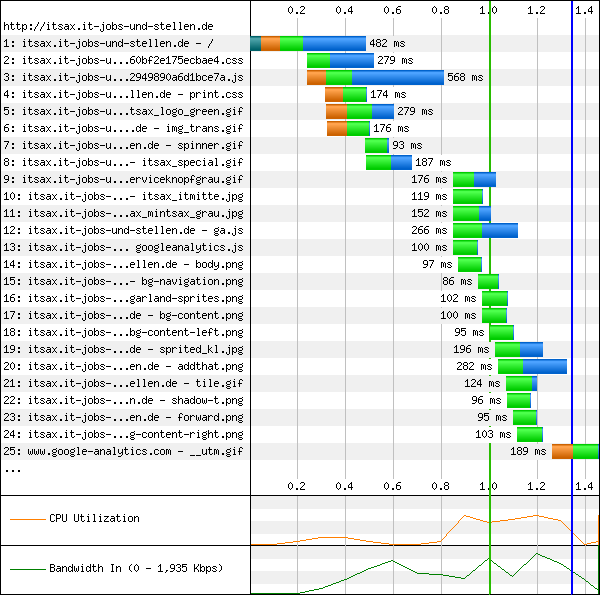
\includegraphics[scale=0.5]{material/end_waterfall.png}
  \caption{Wasserfalldiagramm: Optimierte Webseite}
  \label{fig:endwaterfall}
\end{figure}
%http://www.webpagetest.org/result/110825_5J_1DQHK/
\section{Vergleich}
\begin{center}
    \begin{tabular}{ | p{4cm} | p{1cm} | p{1cm} | p{6cm} |}
    \hline
    Methode & Load Time & TtSR & Kommentar \\ \hline
    \hline
    Ausgangszustand 	& 3,728s  & 2,002s & Der Ausgangszustand ohne Optimierungen. \\ \hline
    JS Aggregation 	& 3,658s  & 1,915s & Bei geringen Aufwand können hier erste Verbesserungen erzielt werden. \\ \hline
    CSS Aggregation 	& 3,577s  & 1,577s & Diese Optimierung sollte auch auf jeden Fall durchgeführt werden. \\ \hline
    Boost Modul 	& 3,233s  & 1,473s & Caching ist Pflicht! Nur in seltenen Ausnahmen ist davon abzusehen. \\ \hline
    Bildkompression verlustfrei 	& 3,640s  & 1,894s & Durch Verringerung der Datenmenge können besonders Handynutzer profitieren.  \\ \hline
    Bildkompression verlustbehaftet 	& 3,255s  & 1,908s & Zusätzliche verlustbehaftete Kompression sorgt oft für schnelleren Seitenaufbau, da große Mengen an Daten eingespart werden können.  \\ \hline
    Drupal 5 Theme Fehler 	& 3,626s  & 1,890s & Durch diese sehr spezielle Optimierung können auch 100ms gewonnen werden.  \\ \hline
    Theme Bilder gesprited 	& 3,707s  & 1,968s & Spriting ist eine gute Möglichkeit Requests zu sparen, macht sich aber leider nicht stark in der Ladezeit bemerkbar.  \\ \hline
    Partnerslideshow 	& 2,749s  & 1,842s & Sehr deutlich wird die Geschwindigkeit durch das asynchrone Nachladen von Inhalten verbessern.  \\ \hline
    Facebook Widget 	& 3,411s  & 1,848s & Besonders bei Inhalten von externen Quellen ist es nützlich die Ladezeiten abzukoppeln.  \\ \hline
    Partneranzeigen 	& 3,871s  & 2,225s & An diesem Beispiel wird deutlich das nachladen nicht unbedingt Verbesserung sein muss, trotzdem ist diese Umprogrammierung nötig um das Caching der Startseite zu ermöglichen.  \\ \hline
    \hline
    Gesamtergebnis 	& 1.354s  & 0.952s & Wenn alle Verbesserungen auf einmal aktiviert werden wird die Webseite dramatisch beschleunigt.  \\ \hline
    
    \hline
    \end{tabular}
\end{center}
 \appendix
%\section{}
%\listoffigures
\cite{*} 
\bibliographystyle{dinat}
\bibliography{bibo}
\end{document}
 
Vorlagen:
\begin{longtable}{|l|l|}
\hline
\rowcolor{Gray}
Falsch&Richtig\\
\hline
Studenten&Studierende\\
\hline
Abschlussprogramm&Degree Seeking Students\\
\hline
Doppeldiplom&Doppelabschluss[programm]\\
\hline
HTWD & HTW Dresden\\
\caption{Deutsche Terminologie}
\label{tb:dt}
\end{longtable}
